% Options for packages loaded elsewhere
\PassOptionsToPackage{unicode}{hyperref}
\PassOptionsToPackage{hyphens}{url}
%
\documentclass[
]{article}
\usepackage{lmodern}
\usepackage{amssymb,amsmath}
\usepackage{ifxetex,ifluatex}
\ifnum 0\ifxetex 1\fi\ifluatex 1\fi=0 % if pdftex
  \usepackage[T1]{fontenc}
  \usepackage[utf8]{inputenc}
  \usepackage{textcomp} % provide euro and other symbols
\else % if luatex or xetex
  \usepackage{unicode-math}
  \defaultfontfeatures{Scale=MatchLowercase}
  \defaultfontfeatures[\rmfamily]{Ligatures=TeX,Scale=1}
\fi
% Use upquote if available, for straight quotes in verbatim environments
\IfFileExists{upquote.sty}{\usepackage{upquote}}{}
\IfFileExists{microtype.sty}{% use microtype if available
  \usepackage[]{microtype}
  \UseMicrotypeSet[protrusion]{basicmath} % disable protrusion for tt fonts
}{}
\makeatletter
\@ifundefined{KOMAClassName}{% if non-KOMA class
  \IfFileExists{parskip.sty}{%
    \usepackage{parskip}
  }{% else
    \setlength{\parindent}{0pt}
    \setlength{\parskip}{6pt plus 2pt minus 1pt}}
}{% if KOMA class
  \KOMAoptions{parskip=half}}
\makeatother
\usepackage{xcolor}
\IfFileExists{xurl.sty}{\usepackage{xurl}}{} % add URL line breaks if available
\IfFileExists{bookmark.sty}{\usepackage{bookmark}}{\usepackage{hyperref}}
\hypersetup{
  pdftitle={Clasificacion},
  pdfauthor={Ignacio Vellido},
  hidelinks,
  pdfcreator={LaTeX via pandoc}}
\urlstyle{same} % disable monospaced font for URLs
\usepackage[margin=1in]{geometry}
\usepackage{graphicx,grffile}
\makeatletter
\def\maxwidth{\ifdim\Gin@nat@width>\linewidth\linewidth\else\Gin@nat@width\fi}
\def\maxheight{\ifdim\Gin@nat@height>\textheight\textheight\else\Gin@nat@height\fi}
\makeatother
% Scale images if necessary, so that they will not overflow the page
% margins by default, and it is still possible to overwrite the defaults
% using explicit options in \includegraphics[width, height, ...]{}
\setkeys{Gin}{width=\maxwidth,height=\maxheight,keepaspectratio}
% Set default figure placement to htbp
\makeatletter
\def\fps@figure{htbp}
\makeatother
\setlength{\emergencystretch}{3em} % prevent overfull lines
\providecommand{\tightlist}{%
  \setlength{\itemsep}{0pt}\setlength{\parskip}{0pt}}
\setcounter{secnumdepth}{-\maxdimen} % remove section numbering
\usepackage{booktabs}
\usepackage{longtable}
\usepackage{array}
\usepackage{multirow}
\usepackage{wrapfig}
\usepackage{float}
\usepackage{colortbl}
\usepackage{pdflscape}
\usepackage{tabu}
\usepackage{threeparttable}
\usepackage{threeparttablex}
\usepackage[normalem]{ulem}
\usepackage{makecell}
\usepackage{xcolor}

\title{Clasificacion}
\author{Ignacio Vellido}
\date{11/24/2020}

\begin{document}
\maketitle

Cargamos los datos

\begin{verbatim}

-- Column specification --------------------------------------------------------
cols(
  Age = col_double(),
  Year = col_double(),
  Positive = col_double(),
  Survival = col_character()
)
\end{verbatim}

Los preprocesamos (estandarización)

Creamos holdout del 90\%

Separamos los datos de las etiquetas

\begin{center}\rule{0.5\linewidth}{0.5pt}\end{center}

\hypertarget{utilizar-el-algoritmo-k-nn-probando-con-diferentes-valores-de-k.-elegir-el-que-considere-muxe1s-adecuado-para-su-conjunto-de-datos.-analice-quuxe9-ocurre-en-los-valores-de-precisiuxf3n-en-training-y-test-con-los-diferentes-valores-de-k.}{%
\subsection{Utilizar el algoritmo k-NN probando con diferentes valores
de k. Elegir el que considere más adecuado para su conjunto de datos.
Analice qué ocurre en los valores de precisión en training y test con
los diferentes valores de
k.}\label{utilizar-el-algoritmo-k-nn-probando-con-diferentes-valores-de-k.-elegir-el-que-considere-muxe1s-adecuado-para-su-conjunto-de-datos.-analice-quuxe9-ocurre-en-los-valores-de-precisiuxf3n-en-training-y-test-con-los-diferentes-valores-de-k.}}

Recordamos los gráficos 1-1 con las clasificaciones, vistos en el EDA.

\begin{center}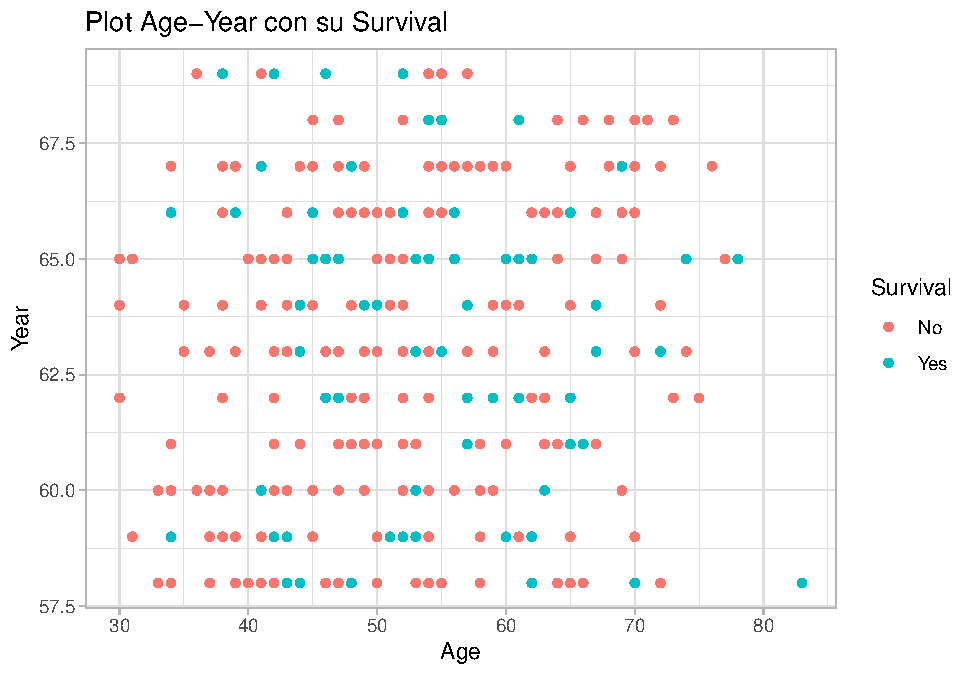
\includegraphics{Clasificacion_files/figure-latex/unnamed-chunk-7-1} \end{center}

\begin{center}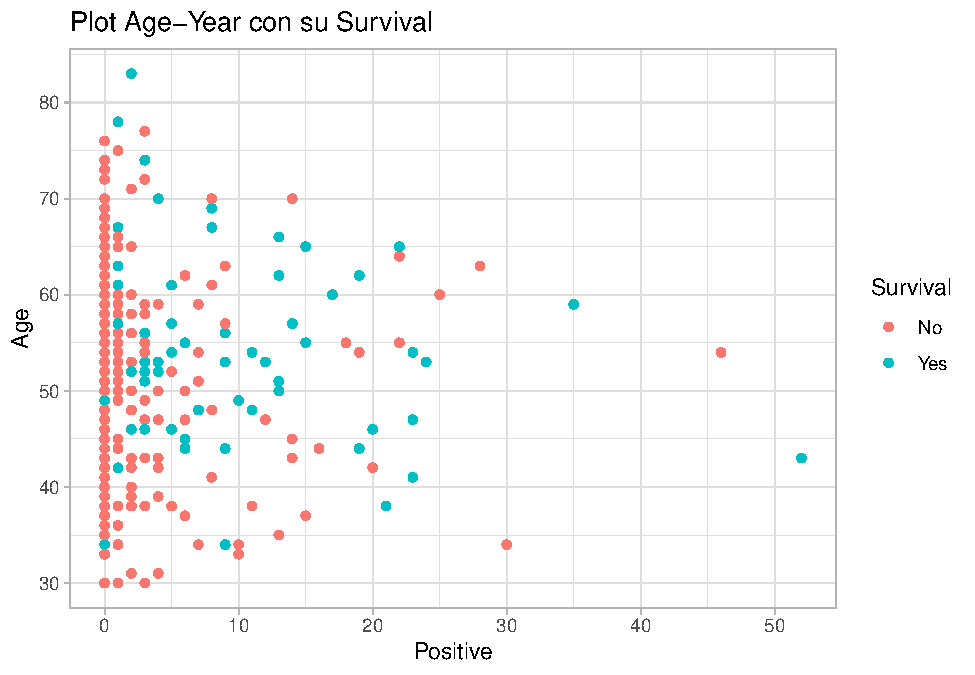
\includegraphics{Clasificacion_files/figure-latex/unnamed-chunk-7-2} \end{center}

\begin{center}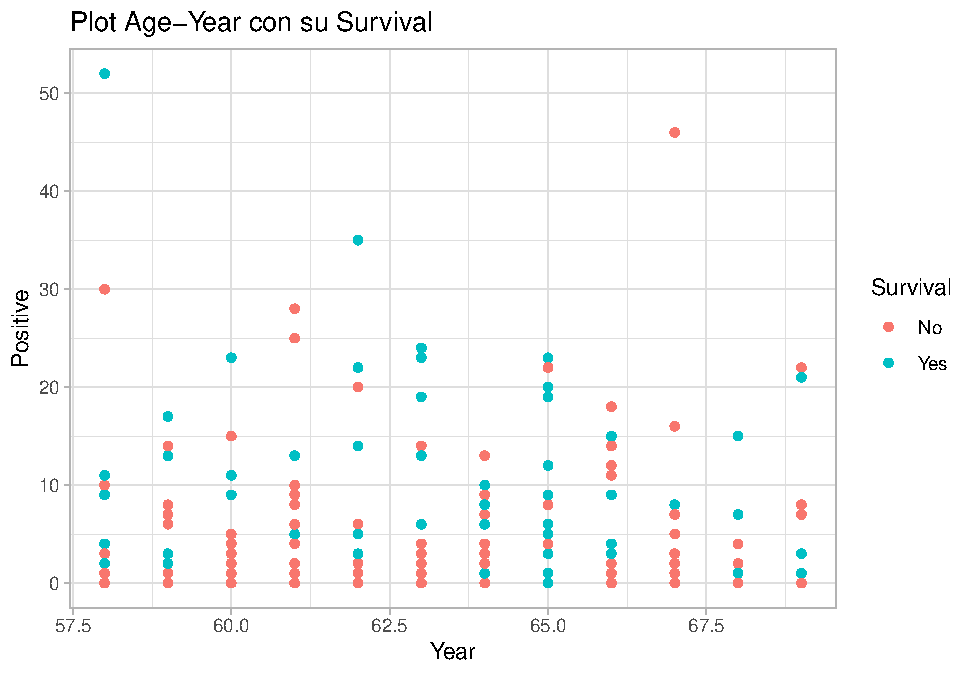
\includegraphics{Clasificacion_files/figure-latex/unnamed-chunk-7-3} \end{center}

\begin{verbatim}
Warning: Unknown or uninitialised column: `color`.
\end{verbatim}

\begin{center}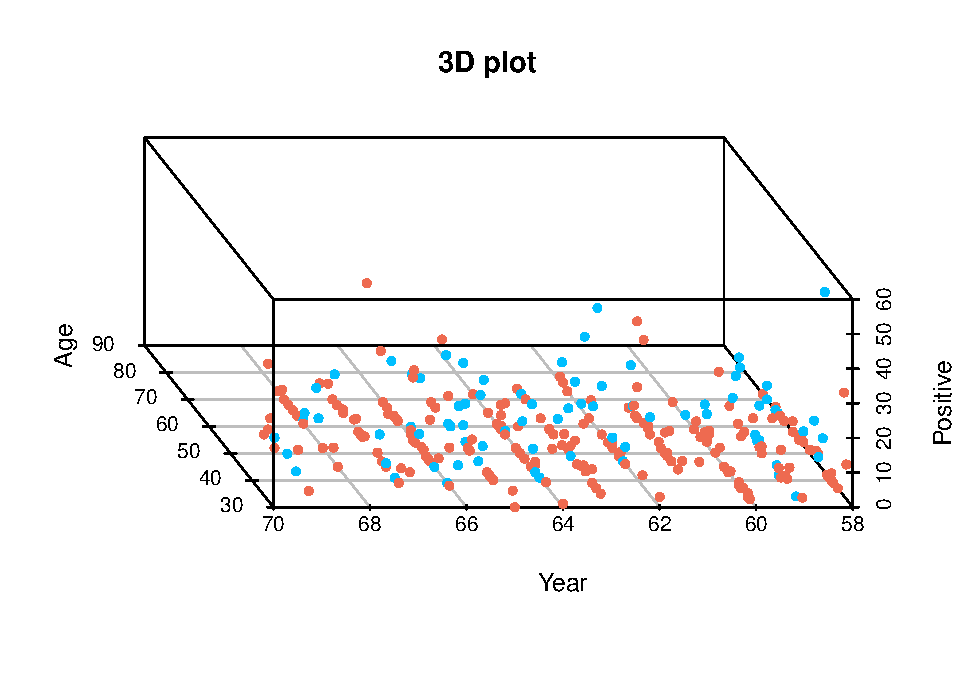
\includegraphics{Clasificacion_files/figure-latex/unnamed-chunk-8-1} \end{center}

\begin{verbatim}
Warning: Unknown or uninitialised column: `color`.
\end{verbatim}

\begin{center}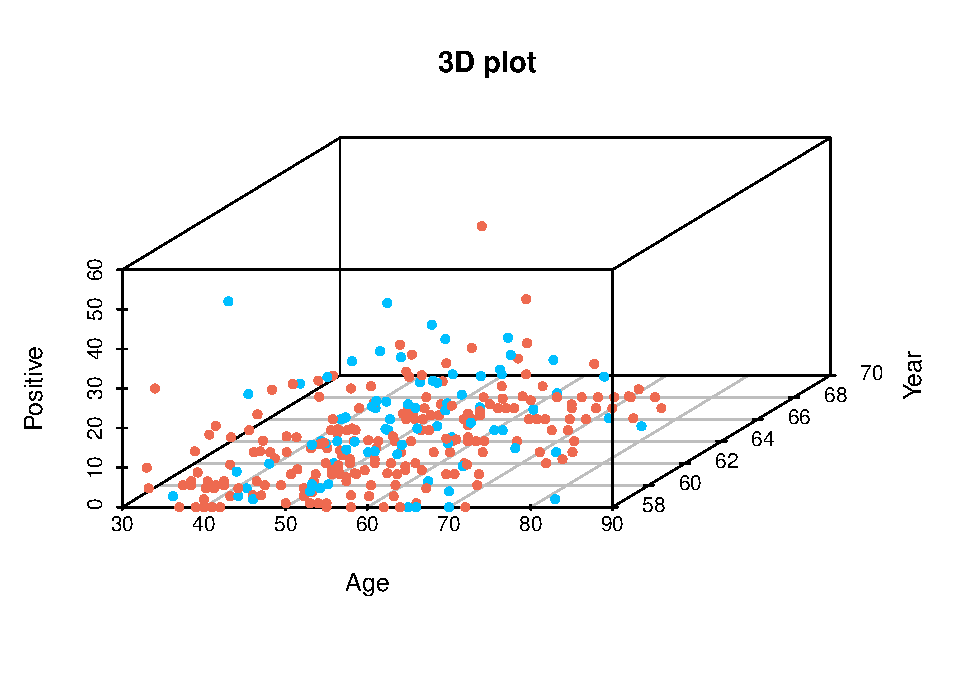
\includegraphics{Clasificacion_files/figure-latex/unnamed-chunk-8-2} \end{center}

De cara a un algoritmo KNN, apreciamos los datos muy entremezclados, con
mayor tendencia a agruparse los no supervivientes que los que sí, pero
nada que nos llame la atención.

Debido a esto vamos a empezar con un valor de K relativamente bajo y
vamos a ir aumentándolo poco a poco. Tenemos que tener cuidado con el
overfitting, eso sí.

\begin{verbatim}
k-Nearest Neighbors 

275 samples
  3 predictor
  2 classes: 'No', 'Yes' 

No pre-processing
Resampling: Cross-Validated (10 fold) 
Summary of sample sizes: 248, 247, 247, 247, 247, 247, ... 
Resampling results across tuning parameters:

  k   Accuracy   Kappa    
   3  0.6947599  0.2034939
   4  0.6832418  0.1615034
   5  0.6884412  0.1100164
   6  0.6879121  0.1426382
   7  0.6950549  0.0983539
   8  0.7165954  0.1496547
   9  0.7240130  0.1881672
  10  0.7164632  0.1470534
  11  0.7277269  0.1753847
  12  0.7203195  0.1708068
  13  0.7241656  0.1767408
  14  0.7313085  0.2015352
  15  0.7422873  0.2320214

Accuracy was used to select the optimal model using the largest value.
The final value used for the model was k = 15.
\end{verbatim}

Recordamos que los datos ya estaban previamente preprocesados
(estandarizados, concretamente)

\begin{verbatim}
       test_labels
knnPred No Yes
    No  26   2
    Yes  1   2
 Accuracy     Kappa 
0.9032258 0.5181347 
\end{verbatim}

Se aprecia que la accuracy en test es ligeramente inferior
(\textasciitilde6 centésimas) a la de training.

\begin{center}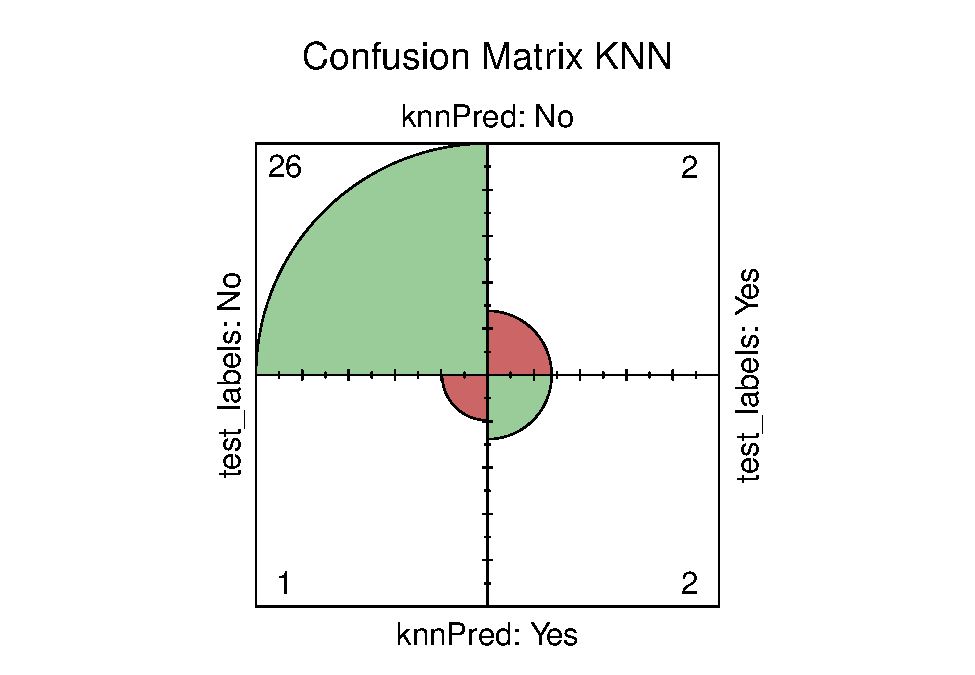
\includegraphics{Clasificacion_files/figure-latex/unnamed-chunk-11-1} \end{center}

Vemos que al estar los datos tan entremezclados ni siquiera con un K
pequeño sobreaprende, es ya con un K medianamente alto (= 13) donde
obtiene mayor accuracy en train.

Probablemente esto se deba a la gran mezcla de los datos, de forma que
necesite la ``opinión'' de un gran número de vecinos para poder predecir
con mayor confianza el nuevo valor.

\begin{center}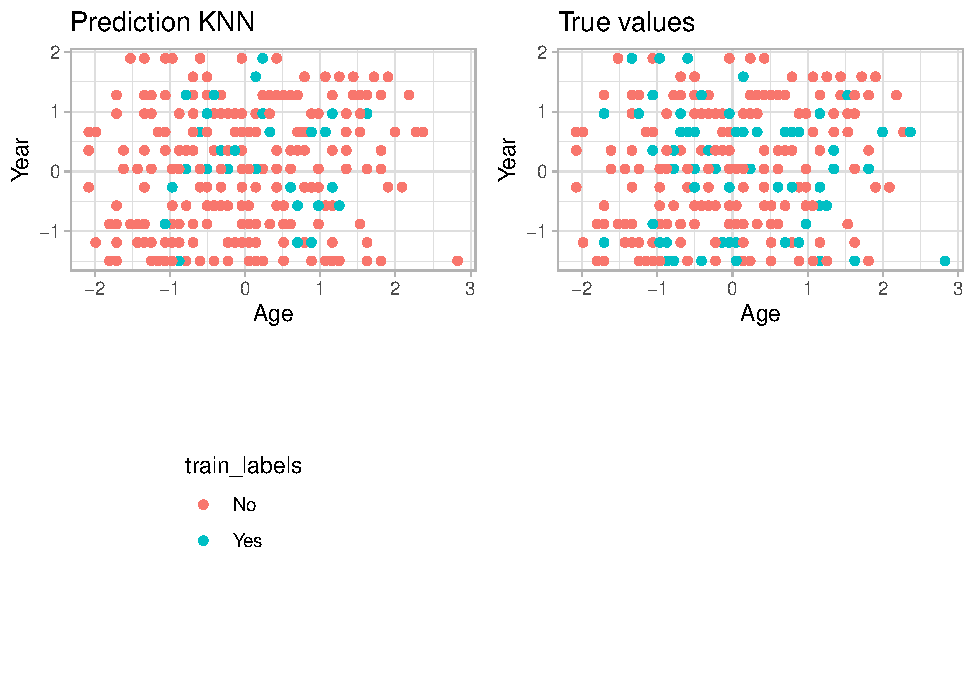
\includegraphics{Clasificacion_files/figure-latex/unnamed-chunk-12-1} \end{center}

Vemos que el uso de un K alto hace que perdamos puntos de Yes.
Probablemente al ser minoría el error cometido clasificándolos como No
es menor y por eso obtiene mejor accuracy.

En principio (a falta de evaluar con CV) creemos que en comparación con
otros algoritmos el hecho de que el dataset este desbalanceado y los
datos muy entremezclados la calidad real (fuera del entrenamiento) no
sea muy buena. Podría ser que en la población se mantega este
desbalanceo en los datos y funcione bien, pero en caso de que no lo sea,
el valor de K tan alto haría que probablemente se tienda a devolver una
predicción de No.

Como habíamos comentado al principio, para el problema que nos atañe
quizás esto podría ser incluso un hecho positivo, ya que los falsos
positivos sería algo que querríamos evitar a toda costa.

\begin{center}\rule{0.5\linewidth}{0.5pt}\end{center}

Podemos también coger otros valores de K en test. Puesto que hemos
obtenido los mejores resultados en training con un K de 13, que es un
valor relativamente alto, podemo probar con uno bajo y uno intermedio (3
y 7)

\begin{verbatim}
k-Nearest Neighbors 

275 samples
  3 predictor
  2 classes: 'No', 'Yes' 

No pre-processing
Resampling: Cross-Validated (10 fold) 
Summary of sample sizes: 248, 247, 248, 248, 247, 247, ... 
Resampling results:

  Accuracy  Kappa    
  0.697619  0.1988554

Tuning parameter 'k' was held constant at a value of 3
\end{verbatim}

\begin{center}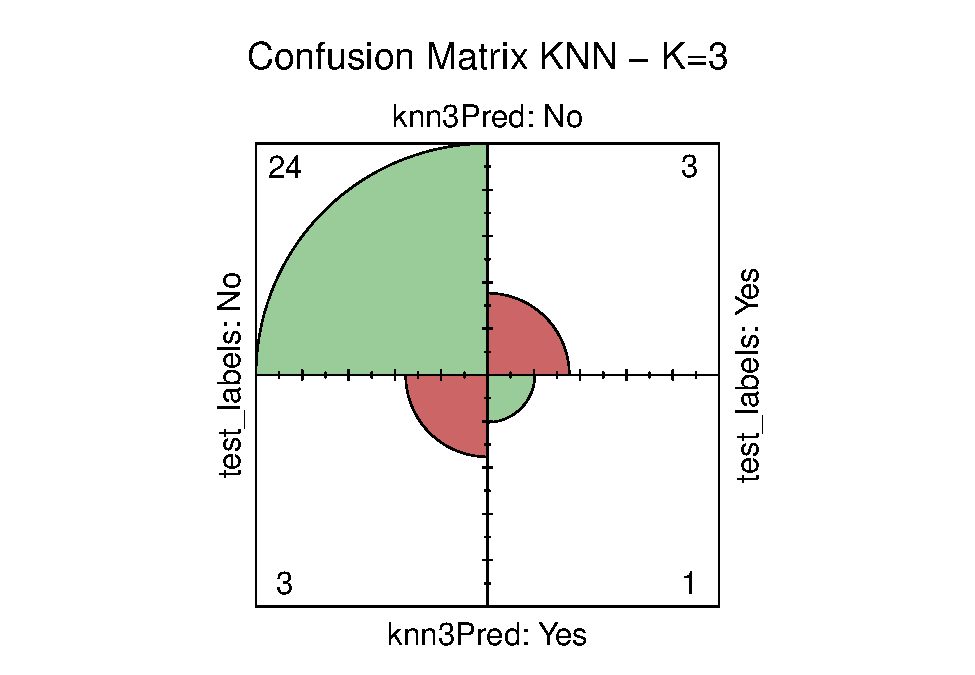
\includegraphics{Clasificacion_files/figure-latex/unnamed-chunk-14-1} \end{center}

\begin{verbatim}
        test_labels
knn3Pred No Yes
     No  24   3
     Yes  3   1
 Accuracy     Kappa 
0.8064516 0.1388889 
\end{verbatim}

\begin{verbatim}
k-Nearest Neighbors 

275 samples
  3 predictor
  2 classes: 'No', 'Yes' 

No pre-processing
Resampling: Cross-Validated (10 fold) 
Summary of sample sizes: 248, 247, 247, 248, 248, 247, ... 
Resampling results:

  Accuracy   Kappa     
  0.6761905  0.08141897

Tuning parameter 'k' was held constant at a value of 7
\end{verbatim}

\begin{center}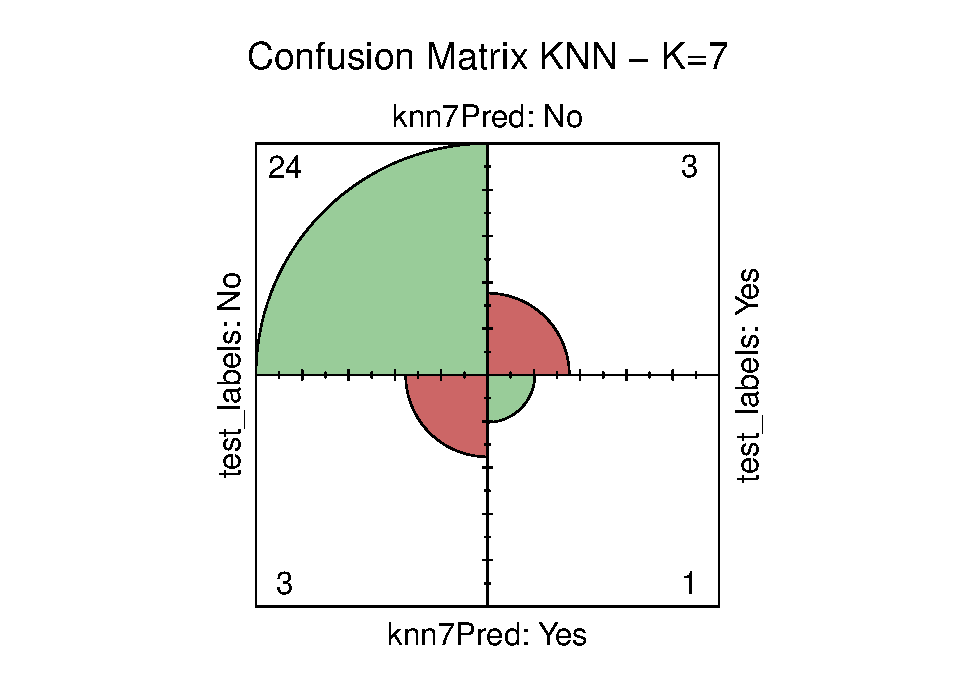
\includegraphics{Clasificacion_files/figure-latex/unnamed-chunk-16-1} \end{center}

\begin{verbatim}
        test_labels
knn7Pred No Yes
     No  24   3
     Yes  3   1
 Accuracy     Kappa 
0.8064516 0.1388889 
\end{verbatim}

K=7 vemos que es el que más sufre al evaluar en test, y ambos (tal y
como nos había indicado CV) tienen una calidad bastante inferior a un
K=13

\begin{center}\rule{0.5\linewidth}{0.5pt}\end{center}

\hypertarget{utilizar-el-algoritmo-lda-para-clasificar.-no-olvide-comprobar-las-asunciones.}{%
\subsection{Utilizar el algoritmo LDA para clasificar. No olvide
comprobar las
asunciones.}\label{utilizar-el-algoritmo-lda-para-clasificar.-no-olvide-comprobar-las-asunciones.}}

Comprobamos asunciones:

1- Distribución aleatoria: No nos queda más remedio que creer que sí.

2- Cada predictor sigue una distribución normal: Ya vimos en el EDA que
esto no era cierto. El test de Shapiro nos demostraba que no y los
QQ-plots nos lo hacían ver claramente. Técnicamente sabiendo esto no
deberíamos usar LDA, pero puesto que esto es un proyecto seguimos
igualmente.

Aún así, las variables Age y Year no parecen seguir una distribución
demasiado ``rara'' (en comparación con una normal), por lo que es
posible que obtengamos resultados decentes.

3- Las clases siguen la misma matriz de covarianza: Solo nos interesa la
diagonal

\begin{verbatim}
New names:
* NA -> ...4
New names:
* NA -> ...4
\end{verbatim}

\begin{verbatim}
Para clase Yes:
      Age      Year  Positive 
0.9176155 1.0113109 1.6788033 
Para clase No:
      Age      Year  Positive 
1.0756415 0.9752581 0.5448553 
\end{verbatim}

Las variables Age y Positive parecen seguir distintas varianzas, lo
aseguramos con un test estadístico.

Puesto que nuestras variables no siguen una distribución normal, no
podemos hacer el test de homogeneidad de Barlett. Utilizamos por tanto
el de Levene

\begin{verbatim}
Age:
\end{verbatim}

\begin{tabular}{l|r|r|r}
\hline
  & Df & F value & Pr(>F)\\
\hline
group & 1 & 1.799898 & 0.1807261\\
\hline
 & 304 & NA & NA\\
\hline
\end{tabular}

\begin{verbatim}
Year:
\end{verbatim}

\begin{tabular}{l|r|r|r}
\hline
  & Df & F value & Pr(>F)\\
\hline
group & 1 & 0.0624405 & 0.8028481\\
\hline
 & 304 & NA & NA\\
\hline
\end{tabular}

\begin{verbatim}
Positive:
\end{verbatim}

\begin{tabular}{l|r|r|r}
\hline
  & Df & F value & Pr(>F)\\
\hline
group & 1 & 18.78912 & 1.99e-05\\
\hline
 & 304 & NA & NA\\
\hline
\end{tabular}

Indicándonos que solo se puede asegurar que la variable Positive no
tiene homogeneidad entre clases diferentes.

Podemos verlo más claro gráficamente

\begin{center}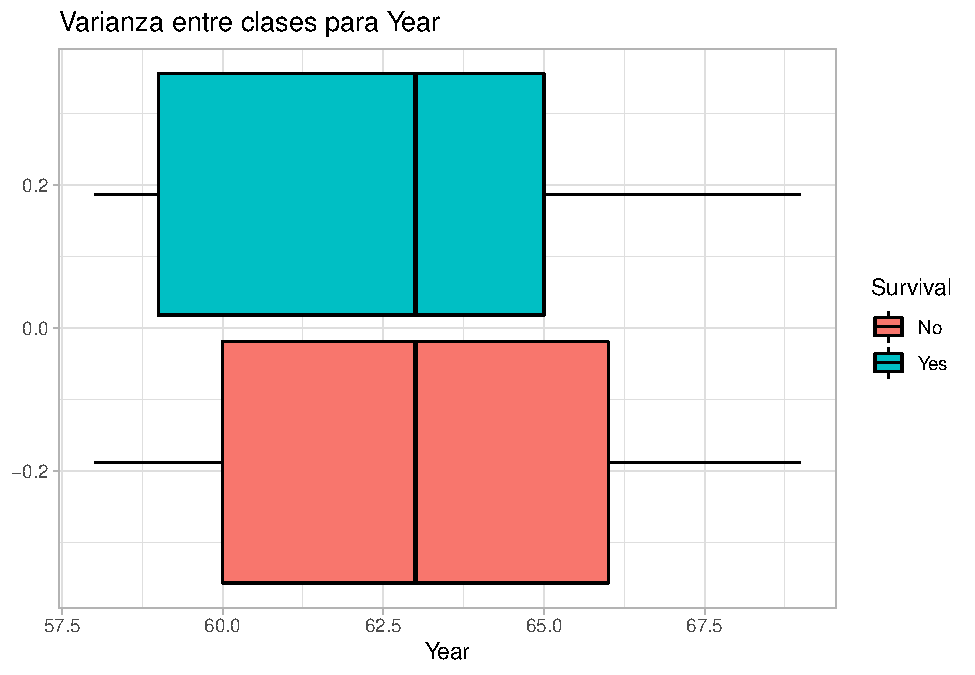
\includegraphics{Clasificacion_files/figure-latex/unnamed-chunk-19-1} \end{center}

\begin{center}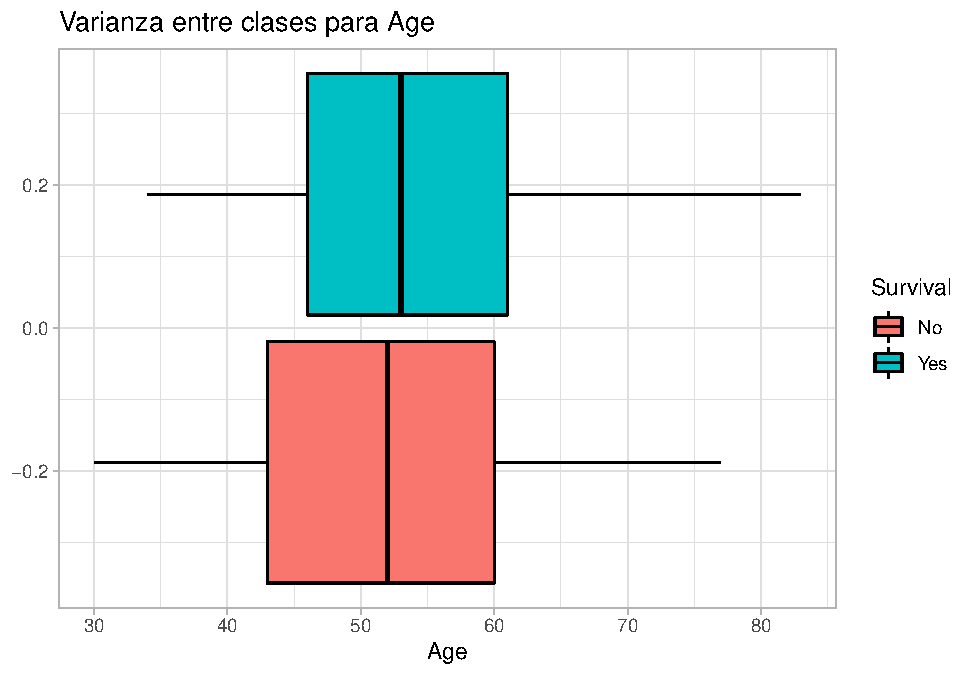
\includegraphics{Clasificacion_files/figure-latex/unnamed-chunk-19-2} \end{center}

\begin{center}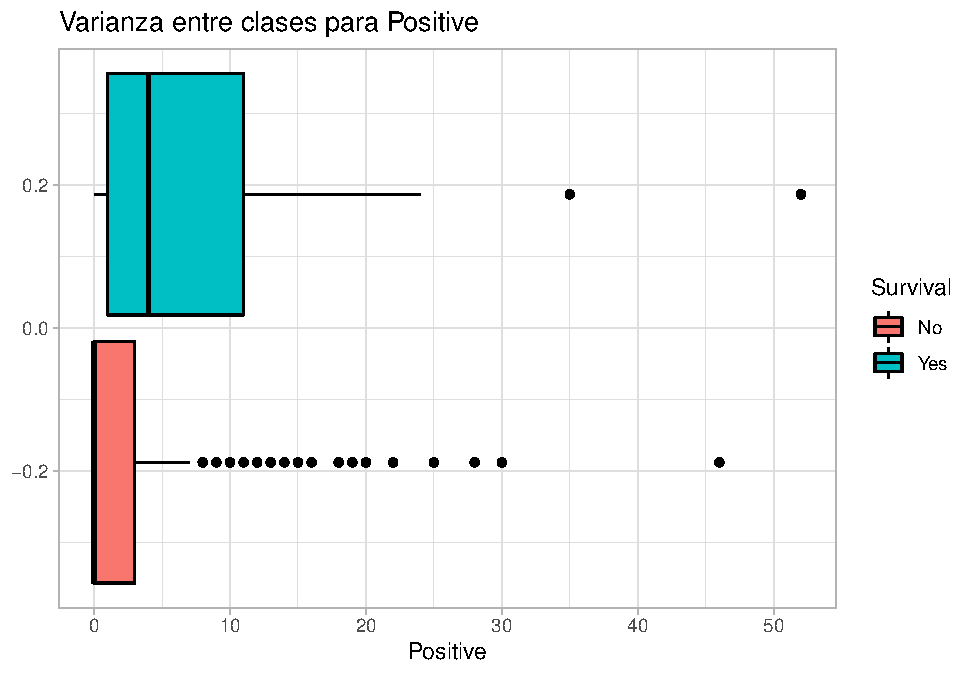
\includegraphics{Clasificacion_files/figure-latex/unnamed-chunk-19-3} \end{center}

Podemos mostrar las varianzas en grafos de elipses:

\begin{center}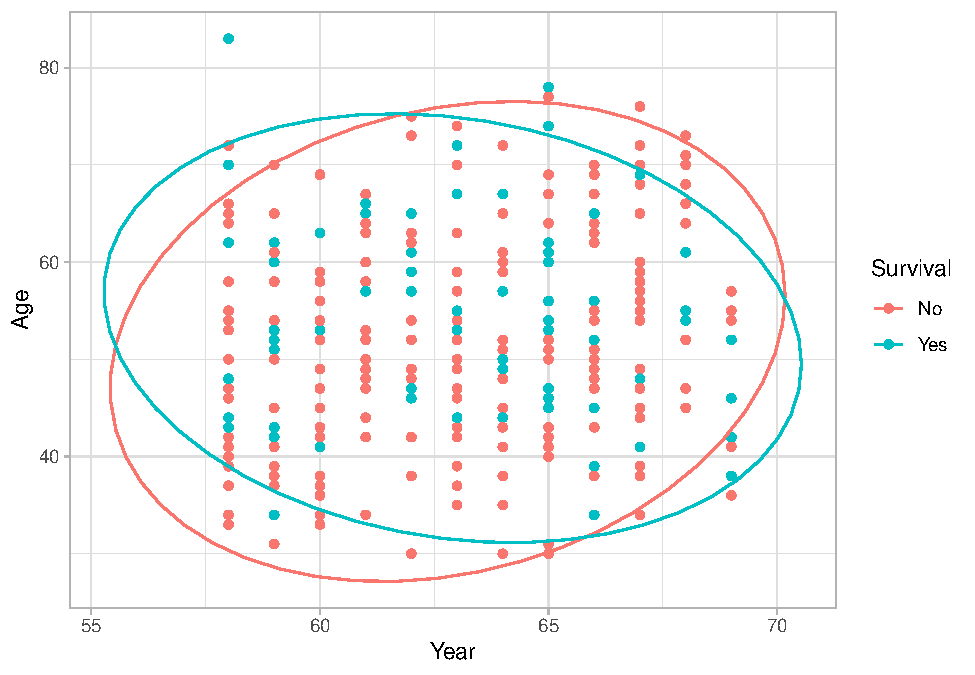
\includegraphics{Clasificacion_files/figure-latex/unnamed-chunk-20-1} \end{center}

\begin{center}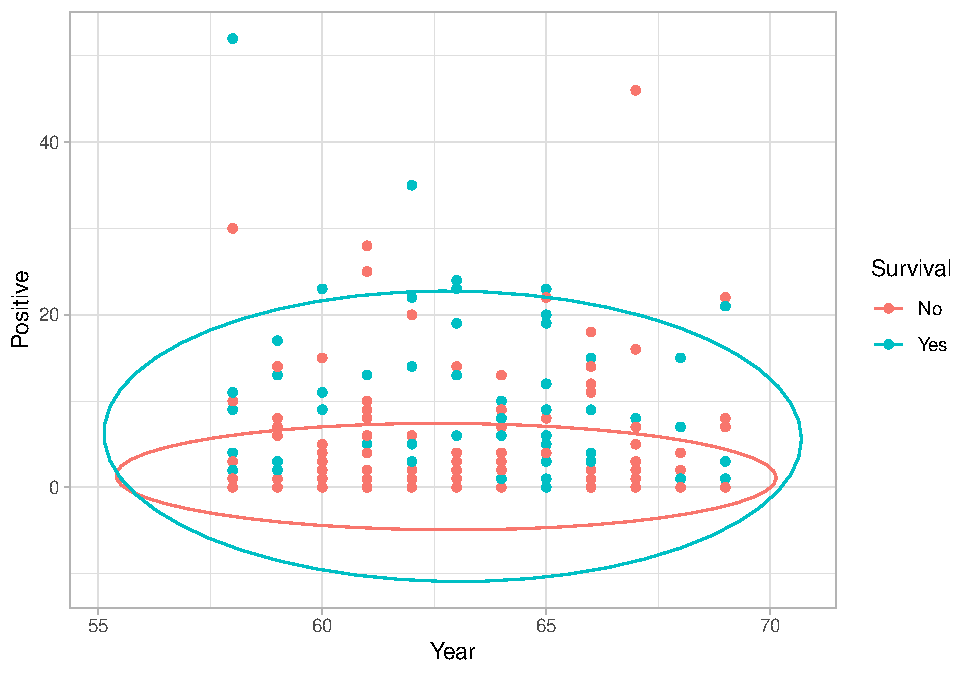
\includegraphics{Clasificacion_files/figure-latex/unnamed-chunk-20-2} \end{center}

\begin{center}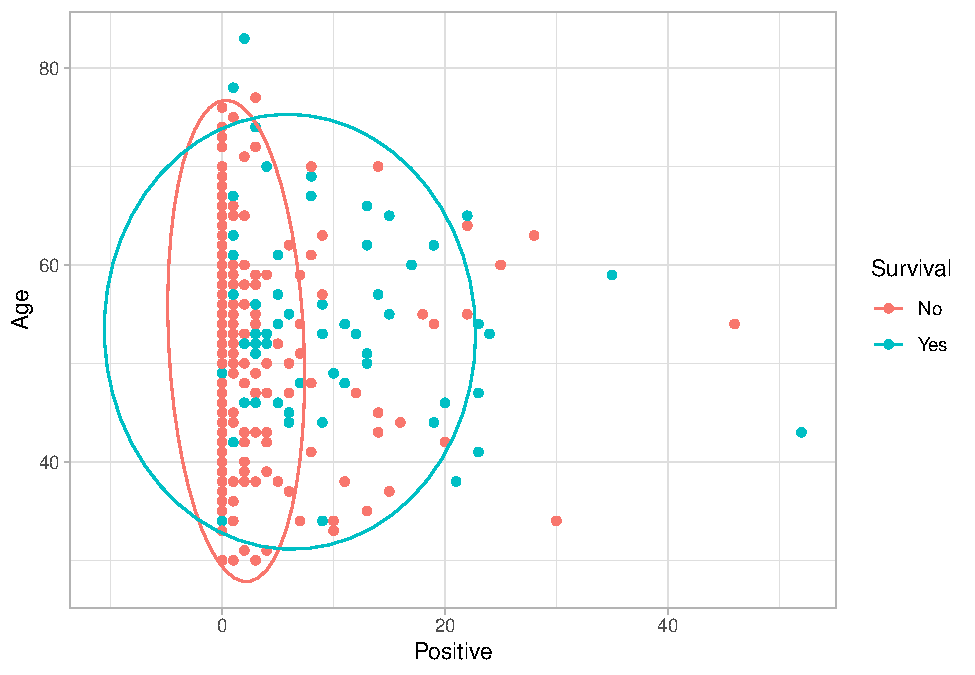
\includegraphics{Clasificacion_files/figure-latex/unnamed-chunk-20-3} \end{center}

Se nota que la causa de que no se rechace el test para esta variable es
la gran cantidad de datos con Positive=0

Por tanto para LDA no podemos hacer uso de la variable Positive, pero sí
de las otras dos.

Aunque solo es recomendable, y no son cualidades necesarias para obtener
solución en LDA: - Tenemos más instancias que predictores, por varios
órdenes de magnitud. - Los predictores son independientes. - No tenemos
varianza cercana a cero

\hypertarget{aplicando-lda}{%
\subsubsection{Aplicando LDA}\label{aplicando-lda}}

\begin{verbatim}
Call:
lda(x, y)

Prior probabilities of groups:
  No  Yes 
0.72 0.28 

Group means:
            Age        Year
No  -0.04141411 0.004845716
Yes  0.11031976 0.021276742

Coefficients of linear discriminants:
            LD1
Age  0.98140853
Year 0.03411981
Cross-Validated (10 fold) Confusion Matrix 

(entries are percentual average cell counts across resamples)
 
          Reference
Prediction No Yes
       No  72  28
       Yes  0   0
                          
 Accuracy (average) : 0.72
\end{verbatim}

Predecimos en test

\begin{verbatim}
       test_labels
ldaPred No Yes
    No  27   4
    Yes  0   0
 Accuracy     Kappa 
0.8709677 0.0000000 
\end{verbatim}

\begin{center}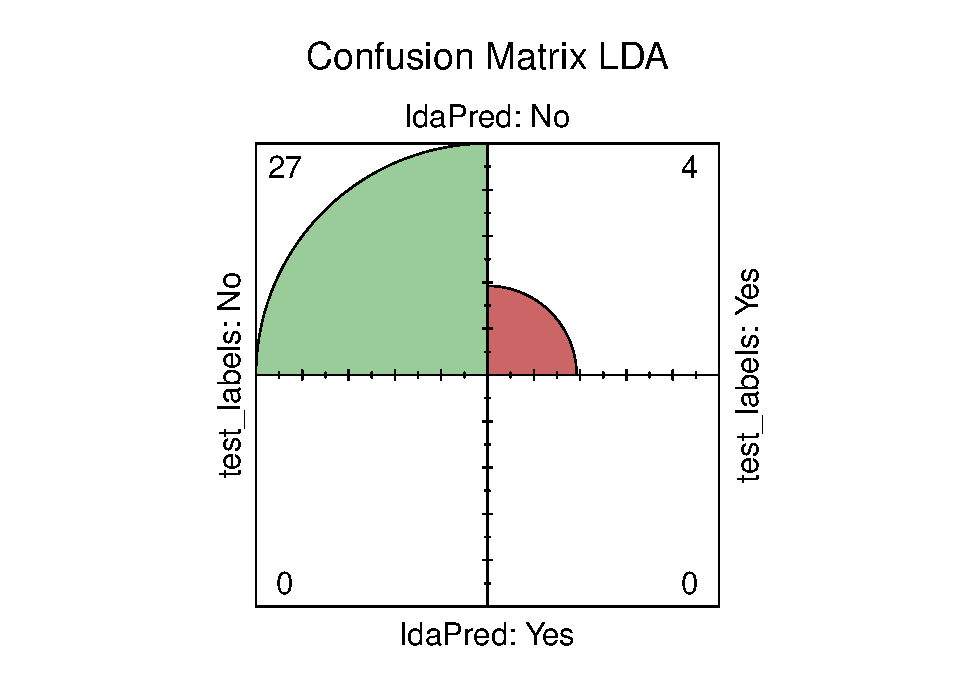
\includegraphics{Clasificacion_files/figure-latex/unnamed-chunk-23-1} \end{center}

En training

\begin{center}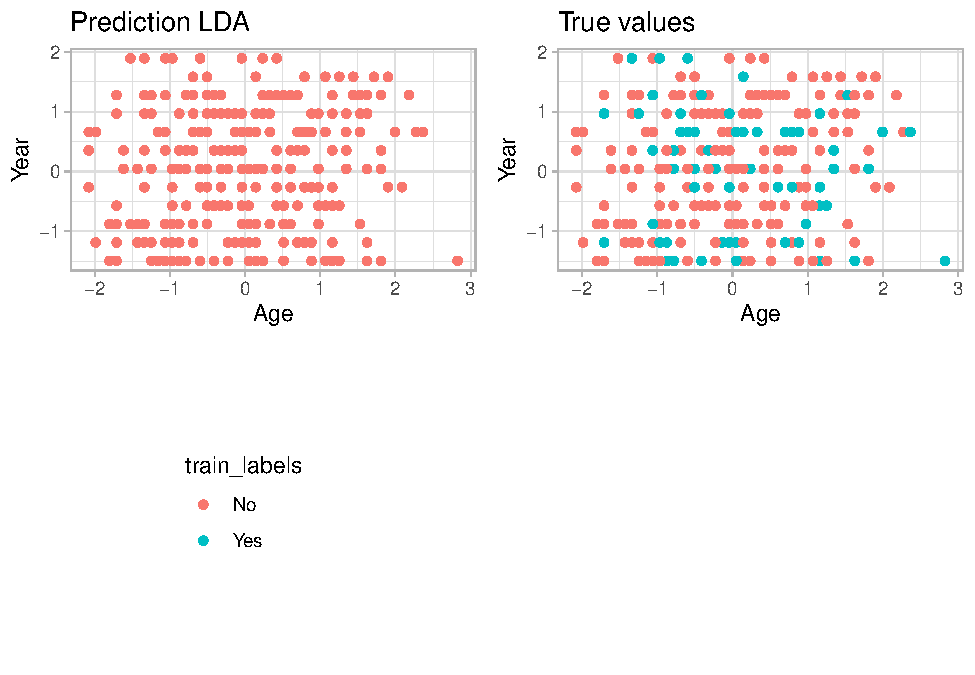
\includegraphics{Clasificacion_files/figure-latex/unnamed-chunk-24-1} \end{center}

Hacemos un plot del ajuste

\begin{verbatim}
New names:
* NA -> ...4
\end{verbatim}

\begin{center}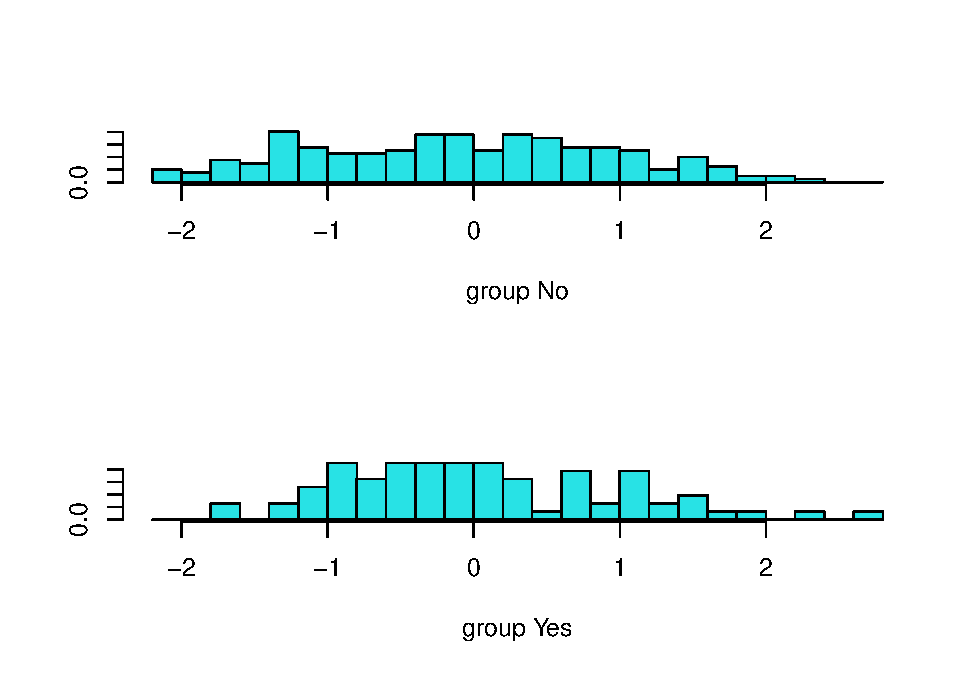
\includegraphics{Clasificacion_files/figure-latex/unnamed-chunk-25-1} \end{center}

\begin{verbatim}
NULL
\end{verbatim}

\begin{center}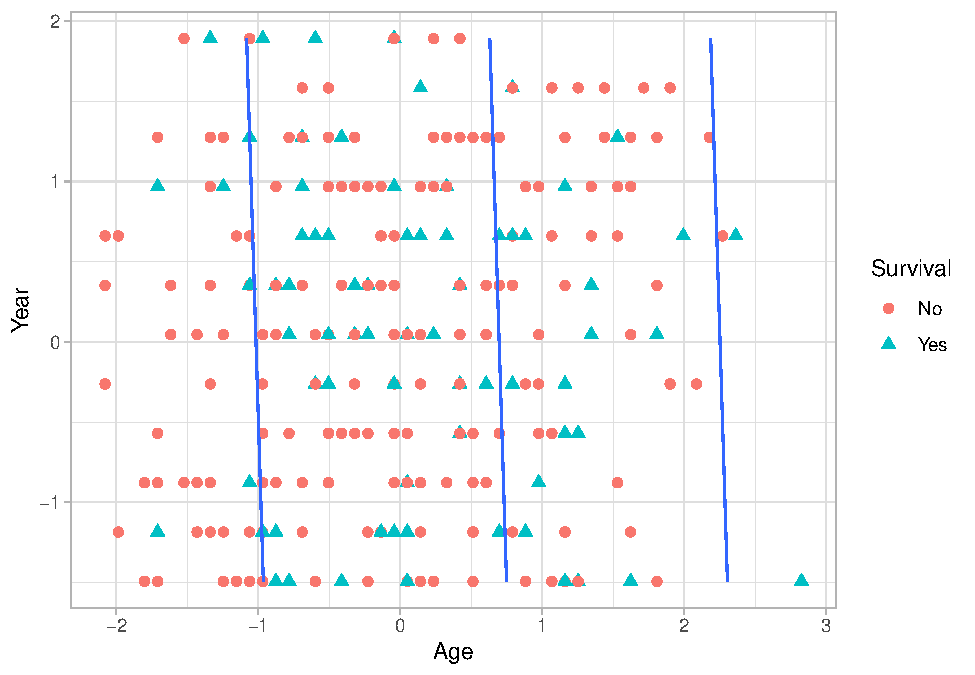
\includegraphics{Clasificacion_files/figure-latex/unnamed-chunk-26-1} \end{center}

(Estamos pintando un contorno 3D y por eso nos salen múltiples líneas en
el gráfico)

Tenemos un dataset bastante desbalanceado, y LDA no predice para la
clase Yes. Con esto se asegura un alto accuracy en nuestro
entrenamiento, pero no asegura de que para datos externos vaya a ser
así. Pese a ello, no nos queda más remedio que suponer que nuestros
datos vienen de la misma muestra aleatoria y por tanto son releventes
para la clasificación.

\begin{center}\rule{0.5\linewidth}{0.5pt}\end{center}

\hypertarget{utilizar-el-algoritmo-qda-para-clasificar.-no-olvide-comprobar-las-asunciones.}{%
\subsection{Utilizar el algoritmo QDA para clasificar. No olvide
comprobar las
asunciones.}\label{utilizar-el-algoritmo-qda-para-clasificar.-no-olvide-comprobar-las-asunciones.}}

QDA tiene las mismas asunciones de LDA salvo que relaja la norma de que
las clases tengan igual covarianza. Esto nos permite usar la variable
Positive que habíamos descartado en LDA.

Por tanto tenemos los requisitos de: - Distribución aleatoria -
Distribución normal

Técnicamente el no cumplir normalidad no imposibilita que se encuentre
solución, pero ya no nos lo asegura.

Además tenemos de forma recomendada que: - El número de predictores debe
ser menor que el número de instancias de cada clase. Cosa que sabemos
que sí por la tabla Yes/No - Los predictores dentro de cada clase no
deben estar correlacionados.

\begin{center}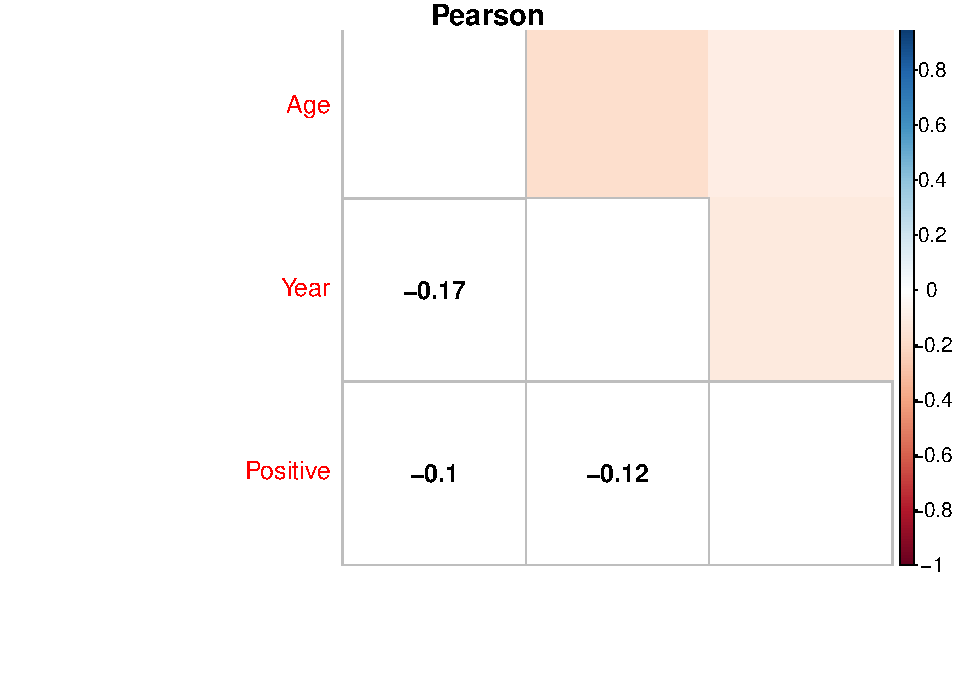
\includegraphics{Clasificacion_files/figure-latex/unnamed-chunk-27-1} \end{center}

\begin{center}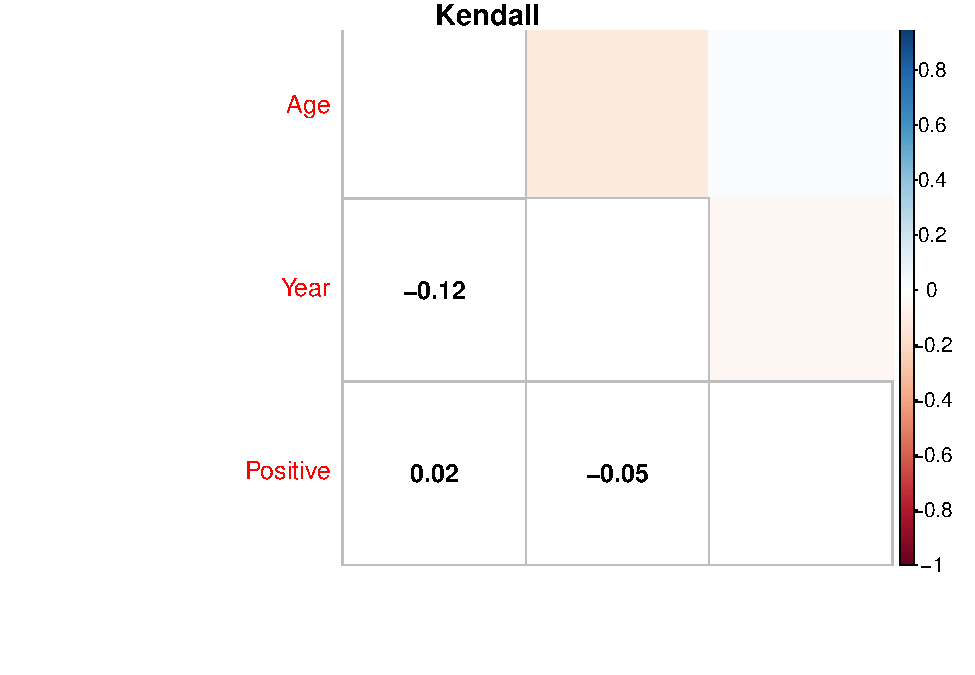
\includegraphics{Clasificacion_files/figure-latex/unnamed-chunk-27-2} \end{center}

\begin{center}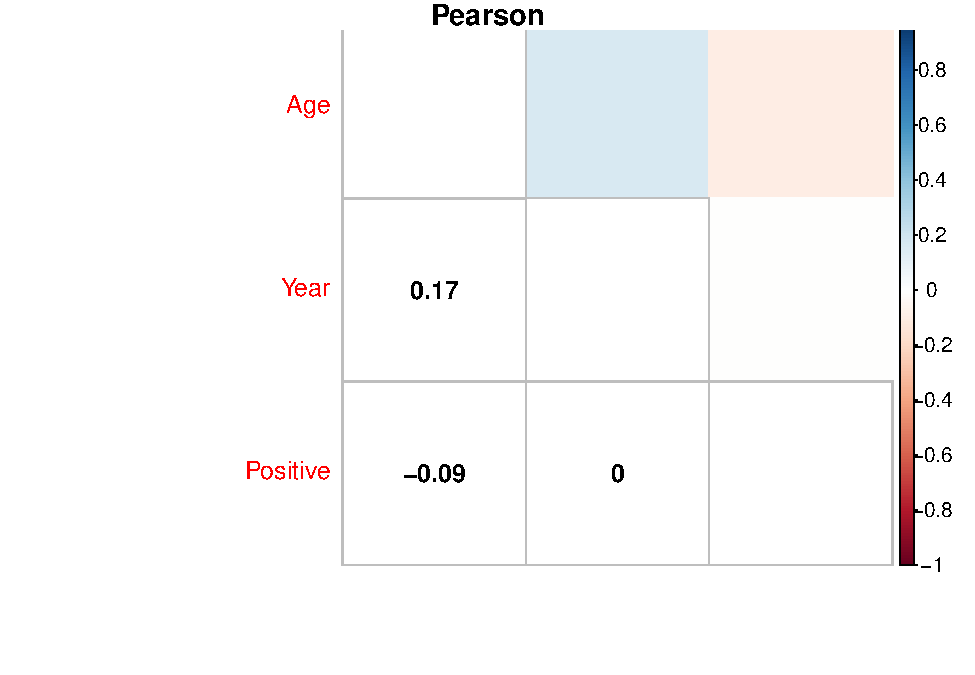
\includegraphics{Clasificacion_files/figure-latex/unnamed-chunk-28-1} \end{center}

\begin{center}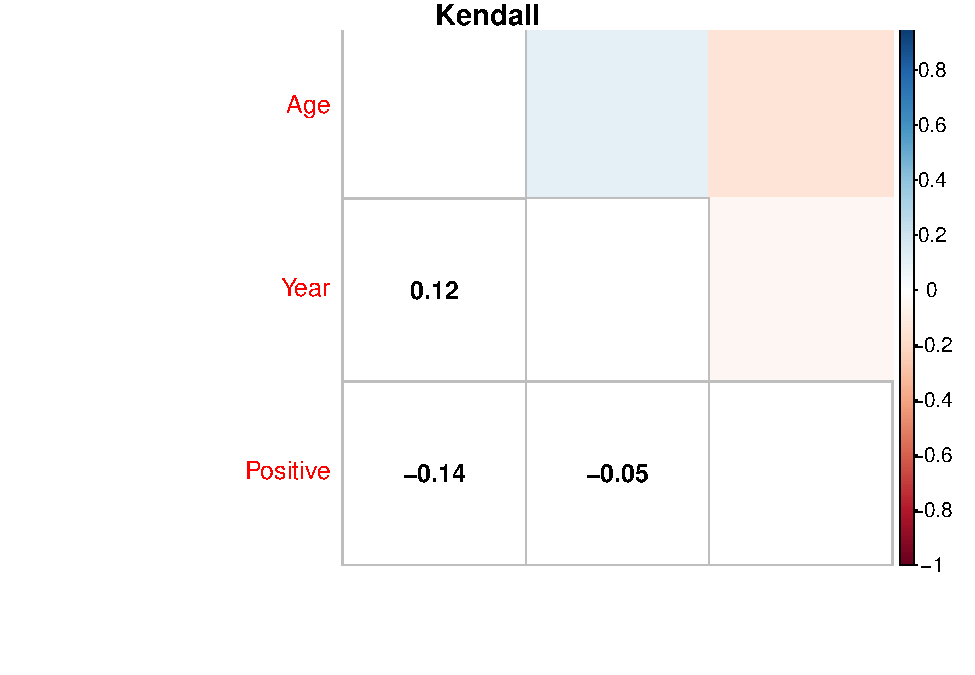
\includegraphics{Clasificacion_files/figure-latex/unnamed-chunk-28-2} \end{center}

No tenemos predictores correlacionados dentro de cada clase.

\begin{center}\rule{0.5\linewidth}{0.5pt}\end{center}

\hypertarget{aplicando-qda}{%
\subsubsection{Aplicando QDA}\label{aplicando-qda}}

\begin{verbatim}
Call:
qda(x, y)

Prior probabilities of groups:
  No  Yes 
0.72 0.28 

Group means:
            Age        Year   Positive
No  -0.04141411 0.004845716 -0.1792534
Yes  0.11031976 0.021276742  0.4804648
Cross-Validated (10 fold) Confusion Matrix 

(entries are percentual average cell counts across resamples)
 
          Reference
Prediction   No  Yes
       No  67.3 21.5
       Yes  4.7  6.5
                            
 Accuracy (average) : 0.7382
\end{verbatim}

\begin{verbatim}
       test_labels
qdaPred No Yes
    No  26   3
    Yes  1   1
 Accuracy     Kappa 
0.8709677 0.2705882 
\end{verbatim}

\begin{center}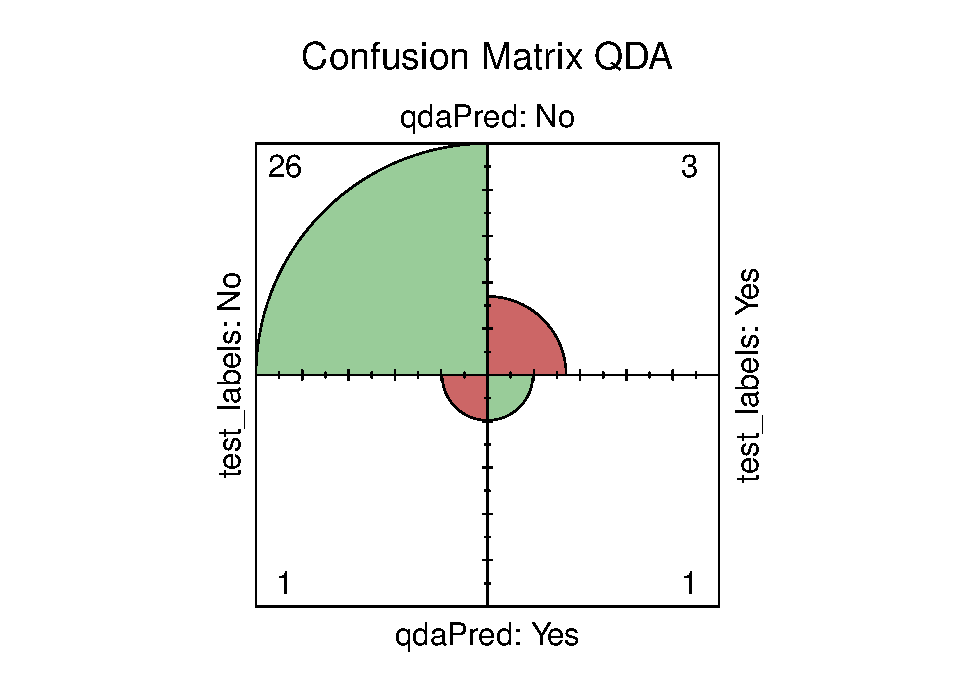
\includegraphics{Clasificacion_files/figure-latex/unnamed-chunk-31-1} \end{center}

En training

\begin{center}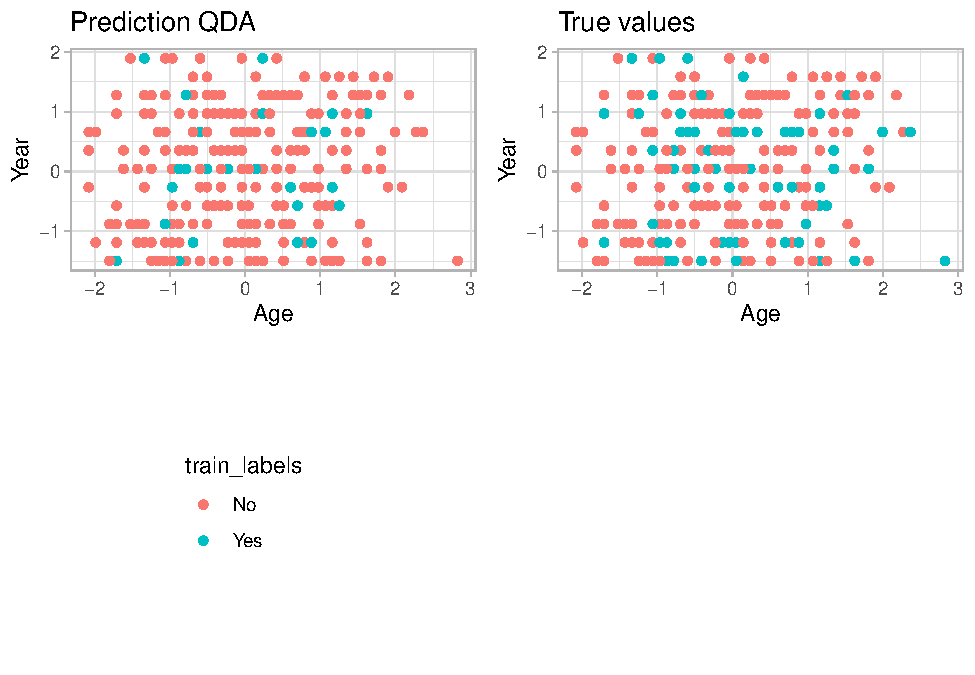
\includegraphics{Clasificacion_files/figure-latex/unnamed-chunk-32-1} \end{center}

Obtenemos resultados extremadamente similares a LDA, pero en este caso
vemos que sí se predice la clase Yes.

\begin{center}\rule{0.5\linewidth}{0.5pt}\end{center}

\hypertarget{comparar-los-resultados-de-los-tres-algoritmos}{%
\subsection{Comparar los resultados de los tres
algoritmos}\label{comparar-los-resultados-de-los-tres-algoritmos}}

Si nos fijamos únicamente en los resultados obtenidos para este
problema, los tres algoritmos obtienen el mismo accuracy en nuestro
conjunto de test. Aunque las etiquetas de este conjunto contienen
elementos de ambas clases, podemos ver que se predice mayoritariamente
la clase No. Como se había mencionado nuestro dataset está bastante
desbalanceado, por lo que era más probable que se predijera esa clase
con mayor facilidad.

(Recordamos que las medidas devueltas en cada algoritmo provienen de un
CV de 10-fold usando el paquete caret)

\begin{verbatim}
Predicciones LDA:
 [1] No No No No No No No No No No No No No No No No No No No No No No No No No
[26] No No No No No No
Levels: No Yes
Predicciones QDA:
 [1] No  No  Yes No  No  No  No  Yes No  No  No  No  No  No  No  No  No  No  No 
[20] No  No  No  No  No  No  No  No  No  No  No  No 
Levels: No Yes
Predicciones KNN:
 [1] No  No  Yes No  No  No  No  Yes No  No  No  No  No  No  No  No  No  Yes No 
[20] No  No  No  No  No  No  No  No  No  No  No  No 
Levels: No Yes

Etiquetas:
 [1] No  No  Yes No  No  No  No  No  Yes No  No  No  No  No  No  No  No  Yes No 
[20] No  No  No  No  No  No  No  No  Yes No  No  No 
Levels: No Yes
\end{verbatim}

\begin{verbatim}
Accuracy KNN:
 Accuracy     Kappa 
0.9032258 0.5181347 

Accuracy LDA:
 Accuracy     Kappa 
0.8709677 0.0000000 

Accuracy QDA:
 Accuracy     Kappa 
0.8709677 0.2705882 
\end{verbatim}

Tenemos la misma accuracy, pero diferentes valores de Kappa, siendo en
general todos bajos.

Pese a esto, puesto que no cumplimos las asunciones necesarias para
asegurarnos resultados en LDA y QDA, para este problema obtaríamos por
usar el algoritmo KNN.

\begin{center}\rule{0.5\linewidth}{0.5pt}\end{center}

Por otro lado, podemos hacer una comparativa general de la calidad de
los algoritmos haciendo uso de las tablas proporcionadas para la
práctica. Para ello, primeramente\ldots{}

Podríamos leer los de training pero para comparar necesitamos los de
test

\begin{verbatim}
Warning: Missing column names filled in: 'X1' [1]
\end{verbatim}

\begin{verbatim}

-- Column specification --------------------------------------------------------
cols(
  X1 = col_character(),
  out_test_knn = col_double(),
  out_test_lda = col_double(),
  out_test_qda = col_double()
)
\end{verbatim}

\begin{tabular}{l|r|r|r}
\hline
X1 & out\_test\_knn & out\_test\_lda & out\_test\_qda\\
\hline
appendicitis & 0.8966667 & 0.8690909 & 0.8109091\\
\hline
australian & 0.6838235 & 0.8579710 & 0.8028986\\
\hline
balance & 0.9024546 & 0.8624101 & 0.9167905\\
\hline
bupa & 0.6865775 & 0.6837924 & 0.5991759\\
\hline
contraceptive & 0.5448653 & 0.5091561 & 0.5173102\\
\hline
haberman & 0.7462069 & 0.7481720 & 0.7512903\\
\hline
hayes-roth & 0.5666667 & 0.5500000 & 0.5875000\\
\hline
heart & 0.6692308 & 0.8481481 & 0.8296296\\
\hline
iris & 0.9642857 & 0.9800000 & 0.9733333\\
\hline
led7digit & 0.7510204 & 0.7420000 & 0.6975000\\
\hline
mammographic & 0.7977698 & 0.8241269 & 0.8194042\\
\hline
monk-2 & 0.9743632 & 0.7703433 & 0.9235535\\
\hline
newthyroid & 0.9071429 & 0.9164502 & 0.9629870\\
\hline
pima & 0.7348861 & 0.7709930 & 0.7412403\\
\hline
tae & 0.3838095 & 0.5245833 & 0.5425000\\
\hline
titanic & 0.7850353 & 0.7760304 & 0.7733032\\
\hline
vehicle & 0.6291452 & 0.7813305 & 0.8522409\\
\hline
vowel & 0.6428571 & 0.6030303 & 0.9191919\\
\hline
wine & 0.6959559 & 0.9944444 & 0.9888889\\
\hline
wisconsin & 0.9735023 & 0.9592185 & 0.9519476\\
\hline
\end{tabular}

\hypertarget{comparativas-1-1-con-wilconxon}{%
\subsubsection{Comparativas 1-1 con
Wilconxon}\label{comparativas-1-1-con-wilconxon}}

LDA vs QDA

\begin{verbatim}
LDA vs QDA: 
    Wilcoxon signed rank exact test

data:  res_norm[, 2] and res_norm[, 1]
V = 96, p-value = 0.7562
alternative hypothesis: true location shift is not equal to 0

R+:   V 
114 
R-:  V 
96 
p-value: [1] 0.7561665
\end{verbatim}

Obtenemos un ranking de 144 para LDA y 96 para QDA, con un p-valor de
0.75 (o nivel de confianza del 25\%).

Esto nos dice que LDA obtiene mejores resultados pero puesto que el
p-value es extremadamente grande no podemos afirmar con garantía
estadística que las diferencias entre los tests sean notorias.

\begin{center}\rule{0.5\linewidth}{0.5pt}\end{center}

LDA vs KNN

\begin{verbatim}
LDA vs KNN: 
    Wilcoxon signed rank exact test

data:  res_norm[, 2] and res_norm[, 1]
V = 120, p-value = 0.5958
alternative hypothesis: true location shift is not equal to 0

R+:  V 
90 
R-:   V 
120 
p-value: [1] 0.5958195
\end{verbatim}

Ahora obtenemos un ranking de 90 para LDA y 120 para QDA, con un p-valor
de 0.59 (o nivel de confianza del 41\%).

Seguimos teniendo un p-valor demasiado grande para poder asegurar con
significación la diferencia.

\begin{center}\rule{0.5\linewidth}{0.5pt}\end{center}

QDA vs KNN

\begin{verbatim}
QDA vs KNN: 
    Wilcoxon signed rank exact test

data:  res_norm[, 2] and res_norm[, 1]
V = 141, p-value = 0.1893
alternative hypothesis: true location shift is not equal to 0

R+:  V 
69 
R-:   V 
141 
p-value: [1] 0.1893482
\end{verbatim}

Por último tenemos un ranking de 69 para LDA y 141 para KNN, con un
p-valor de 0.18 (o nivel de confianza del 82\%).

Ya ahora podemos afirmar al 82\% que los resultados de ambos algoritmos
sí son significativamente diferentes, pero para hacerlo con bastante
seguridad realmente buscaríamos al menos un 95\% de confianza.

\begin{center}\rule{0.5\linewidth}{0.5pt}\end{center}

\hypertarget{comparativa-muxfaltiple-con-friedman}{%
\subsubsection{Comparativa múltiple con
Friedman}\label{comparativa-muxfaltiple-con-friedman}}

\begin{verbatim}

    Friedman rank sum test

data:  as.matrix(results[, 2:4])
Friedman chi-squared = 0.7, df = 2, p-value = 0.7047
\end{verbatim}

El p-value es \textgreater0.05 por lo que no podemos concluir que haya
al menos un par de algoritmos de calidad diferente.

\begin{center}\rule{0.5\linewidth}{0.5pt}\end{center}

\hypertarget{anuxe1lisis-post-hoc-con-holm}{%
\subsubsection{Análisis post-hoc con
Holm}\label{anuxe1lisis-post-hoc-con-holm}}

El resultado del test de Friedman ya nos indica que es post-hoc es
inútil. Los resultados que se obtengan no nos van a asegurar la
diferencia en la calidad de los algoritmos.

Aún así, por completitud en la memoria, aplicamos el test estadístico

\begin{verbatim}
1 = KNN, 2 = LDA, 3 = QDA
    Pairwise comparisons using Wilcoxon signed rank exact test 

data:  as.matrix(results[, 2:4]) and groups 

  1    2   
2 1.00 -   
3 0.53 1.00

P value adjustment method: holm 
\end{verbatim}

Vemos que los p-value son lo más altos posibles, carece de sentido
intentar diferenciar los algoritmos. Aunque podemos notar, tal y como
habíamos visto en los test de Wilcoxon, que la diferencia KNN-QDA
probablemente sea mayor que el resto de parejas.

\end{document}
